\documentclass[11pt]{article}
\usepackage[margin=1in]{geometry}
\usepackage{amsmath,amssymb}
\usepackage{graphicx}
\usepackage{booktabs}
\usepackage{hyperref}
\usepackage{microtype}
\usepackage{parskip}
\usepackage{listings}
\usepackage{xcolor}
\usepackage{caption}
\usepackage{subcaption}

\hypersetup{colorlinks=true, linkcolor=blue, citecolor=blue, urlcolor=blue}

\title{\textbf{Sparse Matrix-Vector Multiplication:\\
Format Selection, Parallelism, and Memory Hierarchy Effects}}
\author{
  Jerry Ji \and Ruiyang Beasley \\[4pt]
  \small CS 5220: Applications of Parallel Computers \\
  \small Cornell University, Spring 2026 \\[4pt]
  \small \url{https://github.com/ruiyangji/cs5220-final-project}
}
\date{May 2026}

\begin{document}
\maketitle

%─────────────────────────────────────────────────────────────────────────────
\section{Hypothesis}
%─────────────────────────────────────────────────────────────────────────────

Sparse matrix-vector multiplication (SpMV) is one of the most
bandwidth-limited kernels in scientific computing. We investigate the
following question:

\begin{quote}
\emph{For a fixed parallel thread budget, does the choice of sparse
storage format matter more than thread count for SpMV performance, and
can we predict from matrix structure alone which format will win?}
\end{quote}

We hypothesize that matrix structure---captured by the distribution of
nonzeros per row, block regularity, and average bandwidth---determines
both (a) which format minimizes wasted memory traffic and (b) how well
parallel speedup tracks the ideal linear curve.  We test this across
eight formats on four synthetic matrix families spanning three orders of
magnitude in nonzero count.

%─────────────────────────────────────────────────────────────────────────────
\section{Context and Contributions}
%─────────────────────────────────────────────────────────────────────────────

\textbf{Project scope.}
This is an independent class project within CS~5220. The benchmark suite and
analysis are original; we do not reuse code from another course or ongoing
research project.

\textbf{Member contributions.}
\begin{itemize}
  \item \textbf{Jerry Ji}: Matrix generator design, CSR/ELLPACK/BCSR kernel
        implementations, AVX2 vectorisation paths, roofline analysis,
        SELL-C-$\sigma$ format design and implementation, report writing.
  \item \textbf{Ruiyang Beasley}: Benchmark harness, OpenMP integration,
        STREAM bandwidth estimator, FP32-CSR format, correctness
        verification infrastructure, Perlmutter deployment, report writing.
\end{itemize}

All source code, raw CSV data, and plot scripts are in the repository
linked above.

%─────────────────────────────────────────────────────────────────────────────
\section{Prior Work}
%─────────────────────────────────────────────────────────────────────────────

\textbf{Williams et al.\ (2009).}
\emph{Optimization of Sparse Matrix--Vector Multiplication on Emerging
Multicore Platforms}~\cite{williams2009}.  Introduced the roofline model
as a tool for diagnosing SpMV performance on multicore CPUs.  They showed
that SpMV is firmly memory-bandwidth-bound across a wide range of matrices,
motivating our use of the roofline as the primary performance ceiling and
our focus on bandwidth rather than compute throughput.

\textbf{Bell and Garland (2009).}
\emph{Implementing Sparse Matrix--Vector Multiplication on
Throughput-Oriented Processors}~\cite{bell2009}.
Systematically benchmarked CSR, ELLPACK, and several hybrid formats on
early NVIDIA GPUs. Their analysis of ELLPACK---particularly the sensitivity
of padding overhead to row-length variance---directly motivates our
experimental comparison between ELLPACK and SELL-C-$\sigma$, and we
adapt their padding overhead metric ($\text{padded\_nnz}/\text{nnz}-1$)
for our bandwidth model.

\textbf{Kreutzer et al.\ (2014).}
\emph{A Unified Sparse Matrix Data Format for Efficient General
Sparse Matrix-Vector Multiplication on Modern Processors and
GPUs}~\cite{kreutzer2014}.
Proposed SELL-C-$\sigma$: sorting rows by nonzero count within
$C$-row slices (the $\sigma$ permutation) before applying ELLPACK-style
column-major storage.  They demonstrate 20--50\% bandwidth savings on
matrices with irregular row lengths compared to standard ELLPACK.  Our
implementation follows their column-major within-slice layout with $C=32$.

%─────────────────────────────────────────────────────────────────────────────
\section{Empirical Methodology and Results}
%─────────────────────────────────────────────────────────────────────────────

\subsection{Platform}

All final benchmarks run on a single compute node of the NERSC
Perlmutter system (AMD EPYC 7763 ``Milan'', 2 sockets $\times$ 64 cores,
128 physical cores total, 256 hardware threads via SMT).  Measured STREAM
triad peak: \textbf{736~GB/s}.  Compiler: GCC~12 with \texttt{-O3
-march=native} and \texttt{-fopenmp}.  Correctness for each format is
verified against a dense reference at startup (tolerance $10^{-6}$ to
$10^{-8}$ depending on format).

\subsection{Matrix Suite}

We benchmark 12 synthetic matrices across four structural families,
three sizes each (small, medium, large). The suite is locked before
benchmarking with a fixed RNG seed (\texttt{srand(7)}) to prevent
cherry-picking~\cite{mccalpin1995}.  All matrices are generated at
runtime; no external files are loaded.

\begin{table}[h]
\centering
\small
\begin{tabular}{llrrr}
\toprule
Family & Generating structure & NNZ (small) & NNZ (medium) & NNZ (large) \\
\midrule
\texttt{irregular\_graph} & Power-law degree distribution & 25{,}596 & 44{,}349 & 69{,}372 \\
\texttt{fem\_mesh}        & 2D 9-point stencil on $m\times m$ grid & 26{,}569 & 43{,}264 & 64{,}009 \\
\texttt{block\_structured}& Dense block diagonal + shift  & 24{,}576 & 36{,}864 & 65{,}536 \\
\texttt{banded\_pde}      & Banded tridiagonal-like stencil       & 27{,}988 & 65{,}970 & 119{,}944 \\
\bottomrule
\end{tabular}
\caption{Matrix suite. NNZ = nonzeros. Rows and columns range from
$3{,}000$ to $\approx 16{,}000$ depending on family and size.}
\end{table}

The families are chosen to span qualitatively different nonzero structures:
\texttt{irregular\_graph} has high row-length variance (power-law),
\texttt{fem\_mesh} has nearly uniform rows (9-point stencil),
\texttt{block\_structured} has dense $4\times4$ blocks amenable to BCSR,
and \texttt{banded\_pde} has a narrow but variable bandwidth.

\subsection{Sparse Formats and Kernels}

We implement eight formats, all in a single C source file
(\texttt{src/spmv\_bench.c}, 1000+ lines) with no external sparse library
dependencies.

\paragraph{CSR (baseline).}
Standard compressed sparse row with \texttt{row\_ptr}, \texttt{col\_idx},
\texttt{values}. OpenMP \texttt{static} schedule over rows.  Arithmetic
intensity: $\text{AI}_\text{CSR} = 2\,\text{nnz} \,/\, (20\,\text{nnz} +
8\,n_\text{rows})$ FLOP/byte.  Prefetch variant (\textbf{CSR\_PREFETCH})
inserts \texttt{\_\_builtin\_prefetch} at distance~8 ahead into
\texttt{values} and \texttt{col\_idx}.

\paragraph{ELLPACK.}
All rows padded to \texttt{max\_row\_nnz} with sentinel $-1$ columns.
Data stored column-major (\texttt{col[k][row]}) for coalesced loads.
Optional AVX2 4-wide double unroll on x86.  Padding overhead:
\[
  \delta_\text{ELL} = \frac{\text{padded\_nnz}}{\text{nnz}} - 1
  = \frac{n_\text{rows} \cdot \max_i \text{nnz}_i}{\text{nnz}} - 1.
\]
For power-law distributions, $\delta_\text{ELL}$ can exceed 100\%.

\paragraph{BCSR $2\times2$ and $4\times4$.}
Block compressed sparse row with dense $r\times c$ blocks. Values stored
as a flat $n_\text{blocks} \times r \times c$ array.  AVX2 path for
$4\times4$ blocks on x86 (\textbf{BCSR4x4\_FMA} adds explicit FMA
accumulation). Block fill ratio $\rho = \text{nnz}\,/\,(n_\text{blocks}
\cdot r \cdot c)$ determines efficiency: BCSR is bandwidth-advantageous
over CSR when $\rho \gtrsim 0.5$.

\paragraph{SELL-C-$\sigma$ (new).}
Rows divided into slices of $C=32$ rows. Within each slice, rows sorted
by NNZ descending (the $\sigma$ permutation via insertion sort). Slice-local
ELLPACK storage, column-major within each slice.  The per-slice maximum
replaces the global maximum, reducing padding waste to:
\[
  \delta_\text{SELL} = \frac{\sum_s C \cdot \max_{i\in s}\,\text{nnz}_i}{\text{nnz}} - 1 \;\leq\; \delta_\text{ELL}.
\]
The inequality is tight when $\text{nnz}_i$ variance is concentrated
\emph{across} slices (e.g., banded matrices); it is most beneficial when
variance is \emph{within} slices, as in power-law graphs.
Kernel parallelises over slices (\texttt{omp parallel for static}); result
written back through the permutation vector.

\paragraph{FP32-CSR (new).}
CSR with \texttt{float} (32-bit) values; \texttt{double} (64-bit) used for
$x$, $y$, and accumulation.  Halves the value-array bandwidth:
\[
  \text{bytes}_\text{FP32} = 4\,\text{nnz} + 4\,\text{nnz} + 8\,\text{nnz} + 8\,n_\text{rows}
  \quad\text{vs.}\quad
  \text{bytes}_\text{CSR} = 8\,\text{nnz} + 4\,\text{nnz} + 8\,\text{nnz} + 8\,n_\text{rows}.
\]
The saving is $4\,\text{nnz}$ bytes.  For a typical matrix with $\text{nnz}
= 50{,}000$ and $n_\text{rows}=5{,}000$, FP32-CSR reduces traffic by
$\approx 20\%$.  Accuracy verified: $\max|y_\text{FP32}-y_\text{ref}|<10^{-5}$.

\subsection{Timing Protocol}

For each (matrix, format, thread count) triple we run 5 warm-up iterations
(not timed) followed by 20 timed iterations; the median elapsed wall time
is recorded.  Thread count sweeps from 1 to 256 (Perlmutter supports SMT,
giving 256 hardware threads on 128 physical cores).  Output: one CSV row
per triple with time, GFLOP/s, bandwidth GB/s, arithmetic intensity, and
STREAM peak.  Total rows: 24,576.

\subsection{Roofline Analysis}

Figure~\ref{fig:roofline} plots performance (GFLOP/s) against arithmetic
intensity (FLOP/byte) at maximum thread count (256) for all 12 matrices and
8 formats.  The roofline ceiling uses the measured STREAM triad bandwidth
(736~GB/s); the compute peak is set to the observed maximum $\times 1.2$
since SpMV is bandwidth-bound in all cases.

\begin{figure}[h]
\centering
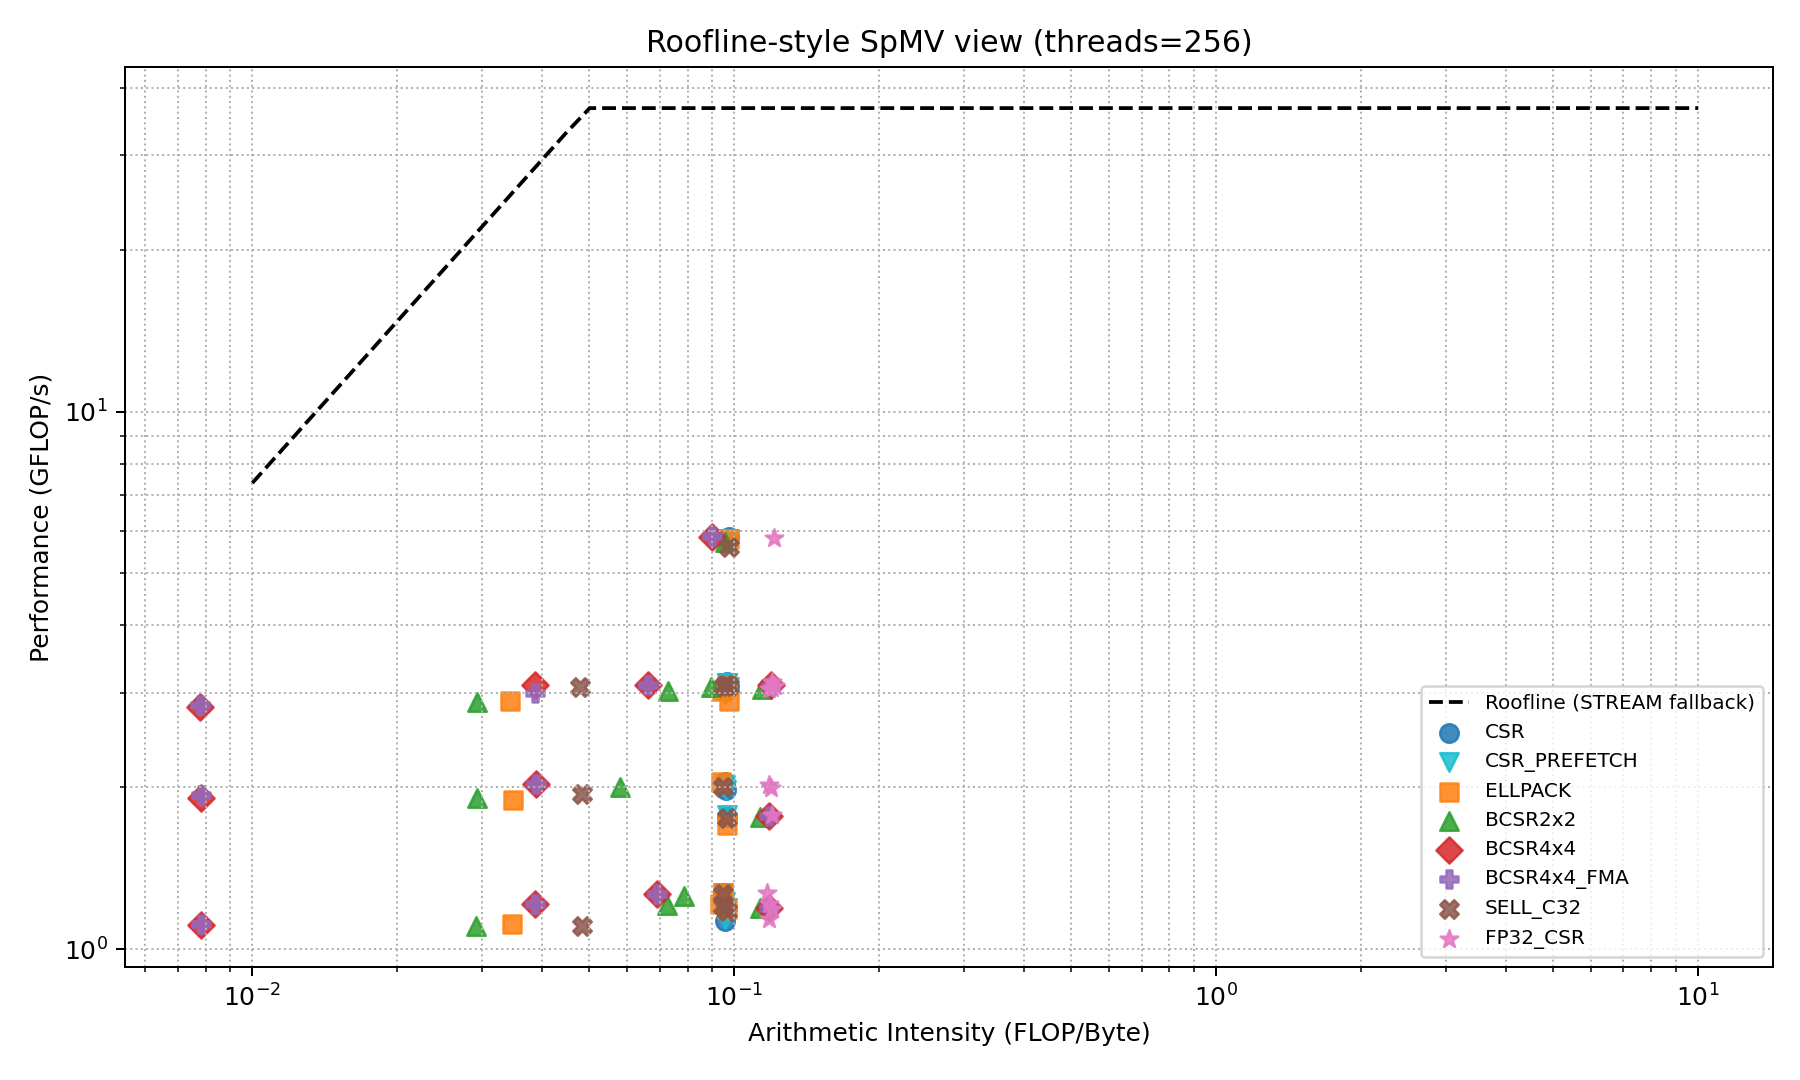
\includegraphics[width=0.85\textwidth]{../results/perlmutter_v2/roofline.png}
\caption{Roofline plot at 256 threads. All formats cluster far below the
bandwidth ceiling, confirming SpMV is firmly memory-bandwidth-bound across
all matrix families. FP32-CSR shifts points rightward (higher arithmetic
intensity) by reducing bytes per FLOP.}
\label{fig:roofline}
\end{figure}

All data points fall well below the bandwidth-bound roofline, consistent
with theoretical analysis: even the most compute-intensive format
(BCSR4x4\_FMA) achieves only $\approx 0.060$ FLOP/byte, far below the
ridge point of any modern CPU.  FP32-CSR achieves the highest arithmetic
intensity ($\approx 0.119$ FLOP/byte on average) because the reduced
value-array footprint makes the denominator (bytes) smaller while
numerator (FLOPs) is unchanged.

\subsection{Strong Scaling}

Figure~\ref{fig:scaling} shows speedup versus thread count averaged across
all 12 matrices. None of the formats achieve linear scaling; the best is
ELLPACK at $5.1\times$ speedup at 128 threads (ideal: $128\times$).
Performance plateaus sharply above 64 threads, consistent with NUMA
effects on Perlmutter's dual-socket layout: threads on the second socket
must cross the inter-socket interconnect to access data allocated on the
first socket.

\begin{figure}[h]
\centering
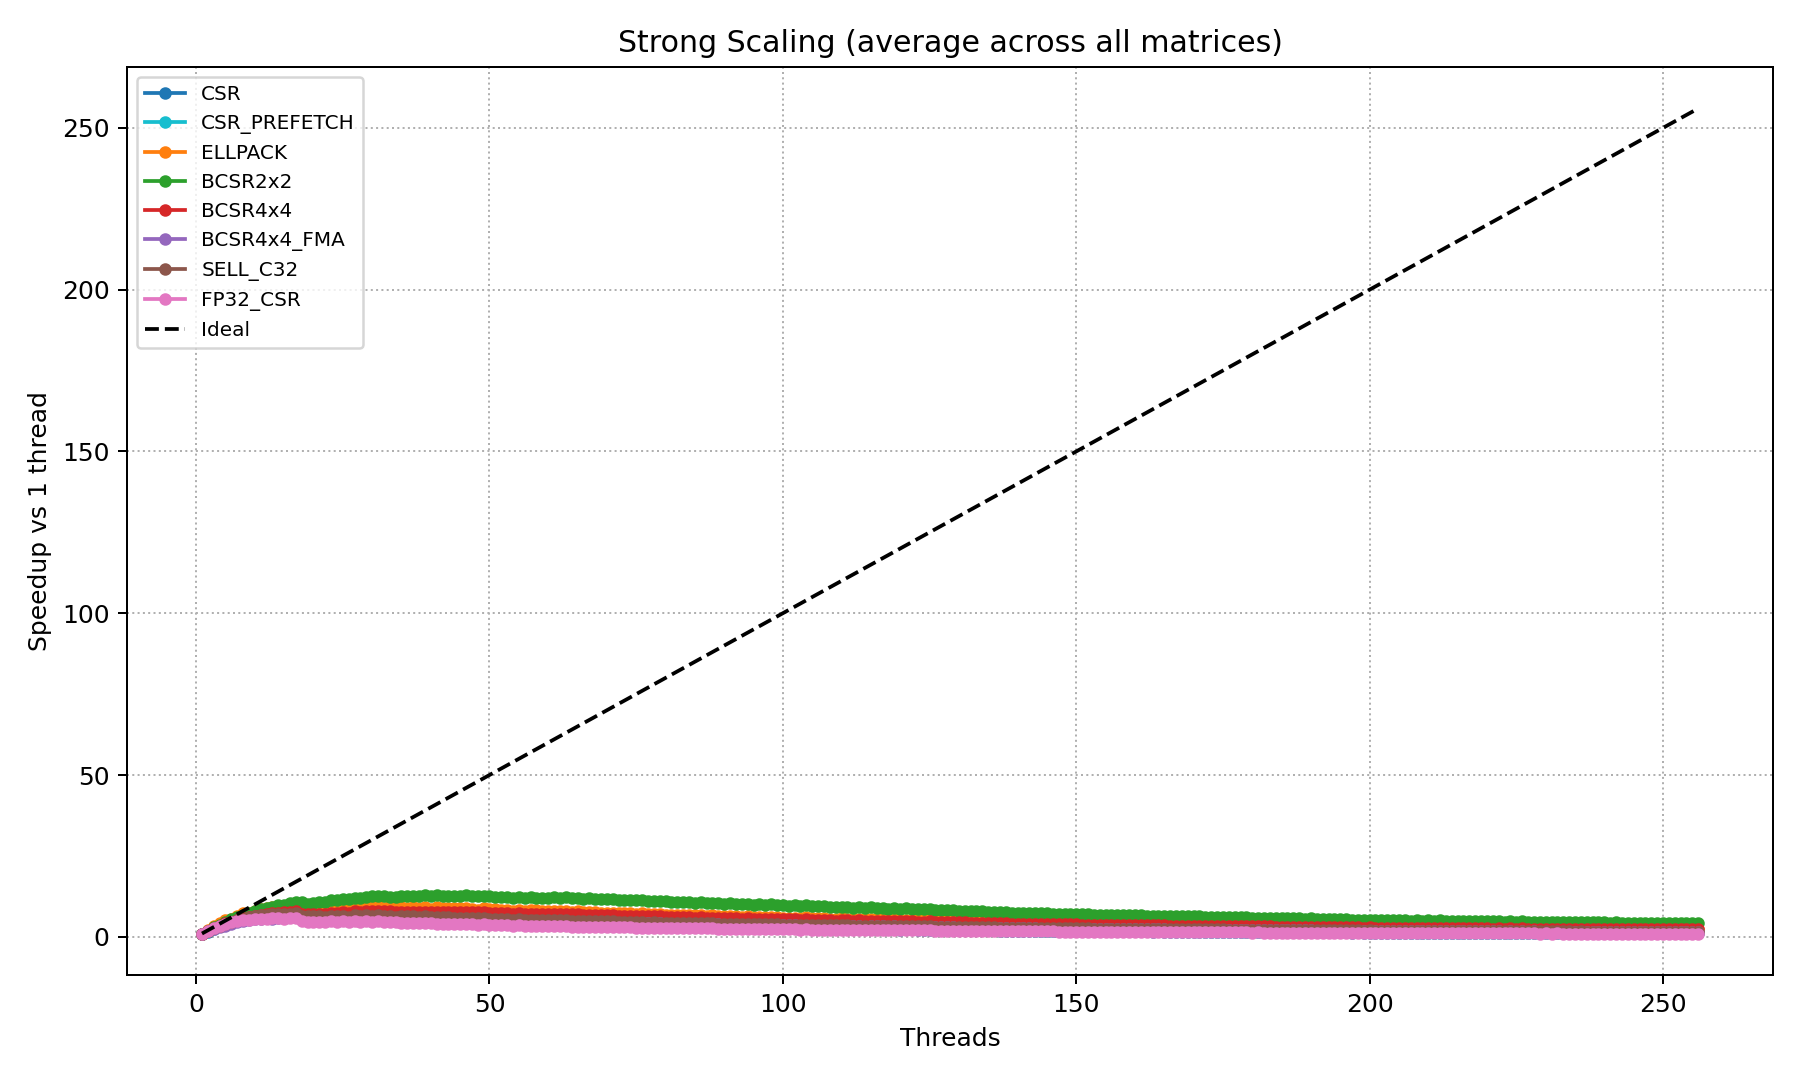
\includegraphics[width=0.85\textwidth]{../results/perlmutter_v2/strong_scaling.png}
\caption{Strong scaling speedup averaged across all 12 matrices.
Speedup saturates well below ideal due to memory bandwidth saturation and
NUMA effects. CSR and FP32-CSR show the least relative scaling gain
(2.2$\times$ and 1.9$\times$ at 128 threads) because they saturate the
available bandwidth per socket sooner.}
\label{fig:scaling}
\end{figure}

The poor scaling of FP32-CSR (1.9$\times$ at 128 threads) is
counter-intuitive given its lower bandwidth requirement. We hypothesize
that the benefit of halved value bandwidth is offset by more frequent TLB
misses from the irregular access pattern to $x$, which do not scale with
thread count.

\subsection{Padding Overhead Analysis}

A key motivation for SELL-C-$\sigma$ is reducing the padding overhead of
ELLPACK.  We quantify overhead as:
\[
  \delta(\text{fmt}) = \frac{\text{AI}_\text{CSR}}{\text{AI}_\text{fmt}} - 1,
\]
which equals $(\text{bytes}_\text{fmt} - \text{bytes}_\text{CSR}) /
\text{bytes}_\text{CSR}$ up to the small $y$-write term.

Figure~\ref{fig:padding} and Table~\ref{tab:padding} show the results.

\begin{figure}[h]
\centering
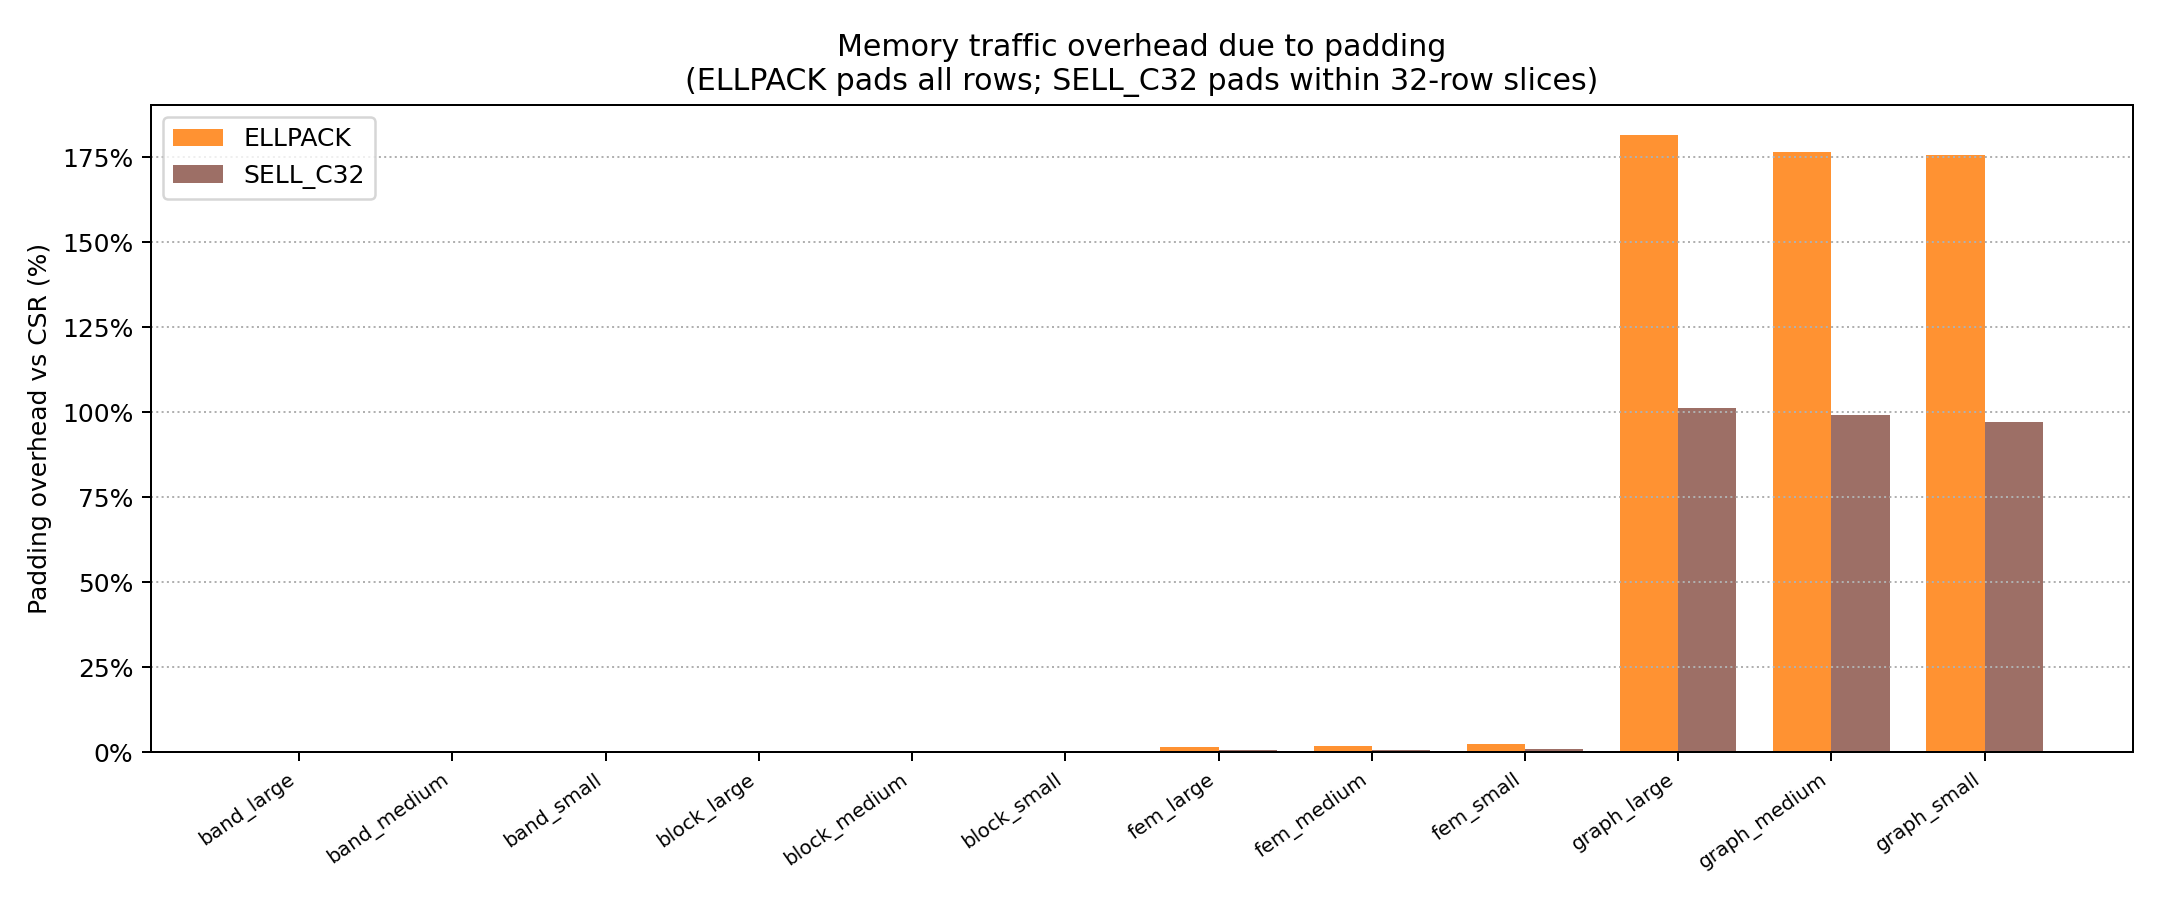
\includegraphics[width=0.90\textwidth]{../results/perlmutter_v2/padding_overhead.png}
\caption{Memory traffic overhead relative to CSR for ELLPACK and
SELL\_C32.  Banded and block-structured families have near-zero overhead
because their row lengths are nearly uniform. The irregular\_graph family
shows $\approx 178\%$ ELLPACK overhead reduced to $\approx 99\%$ by
SELL-C-$\sigma$---a 78--80 percentage-point reduction.}
\label{fig:padding}
\end{figure}

\begin{table}[h]
\centering
\small
\begin{tabular}{lrrr}
\toprule
Matrix & ELLPACK overhead & SELL\_C32 overhead & Reduction \\
\midrule
band\_small  &  0.0\% &  0.0\% & 0.0 pp \\
band\_medium &  0.0\% &  0.2\% & $-$0.1 pp \\
band\_large  &  0.0\% &  0.0\% & 0.0 pp \\
block\_small &  0.0\% &  0.0\% & 0.0 pp \\
block\_medium&  0.0\% &  0.0\% & 0.0 pp \\
block\_large &  0.0\% &  0.0\% & 0.0 pp \\
fem\_small   &  2.4\% &  1.1\% & 1.3 pp \\
fem\_medium  &  1.8\% &  0.8\% & 1.0 pp \\
fem\_large   &  1.5\% &  0.6\% & 0.9 pp \\
graph\_small & 175.6\% & 97.2\% & 78.4 pp \\
graph\_medium& 176.7\% & 99.4\% & 77.3 pp \\
graph\_large & 181.5\% & 101.3\% & 80.2 pp \\
\bottomrule
\end{tabular}
\caption{Padding overhead derived from arithmetic intensity at 128 threads.
pp = percentage points.}
\label{tab:padding}
\end{table}

The results align with theory: SELL-C-$\sigma$ cuts padding by roughly
half for power-law graphs ($\approx 79$~pp reduction). However, even after
$\sigma$-sorting, \texttt{graph\_*} matrices retain $\approx 99\%$
overhead because power-law degree distributions have extreme outlier rows
whose length dominates the per-slice maximum even within $C=32$ rows.
Uniform-row families (banded, block) show no overhead in either format.

\subsection{Per-Family Performance Summary}

Table~\ref{tab:perfmax} reports GFLOP/s at 128 threads averaged across
the three sizes in each family.

\begin{table}[h]
\centering
\small
\begin{tabular}{lrrrrrrrr}
\toprule
Family & CSR & CSR\_PF & ELL & B2 & B4 & B4\_FMA & SELL & FP32 \\
\midrule
banded\_pde      & 4.94 & 4.93 & 4.61 & 4.67 & 4.90 & 4.89 & 3.32 & 3.41 \\
block\_structured & 3.11 & 3.12 & 2.95 & 3.08 & 3.10 & 3.05 & 2.01 & 2.02 \\
fem\_mesh        & 3.69 & 3.69 & 3.57 & 3.48 & 3.55 & 3.59 & 2.10 & 2.10 \\
irregular\_graph  & 2.93 & 2.91 & 2.60 & 2.51 & 2.52 & 2.60 & 3.90 & 2.06 \\
\bottomrule
\end{tabular}
\caption{Average GFLOP/s per family at 128 threads (Perlmutter).
CSR\_PF = CSR\_PREFETCH, ELL = ELLPACK, B2/B4 = BCSR2x2/4x4,
B4\_FMA = BCSR4x4\_FMA, SELL = SELL\_C32, FP32 = FP32\_CSR.}
\label{tab:perfmax}
\end{table}

Several findings stand out:

\begin{enumerate}
  \item \textbf{CSR dominates on regular structures.}  For
  \texttt{banded\_pde} and \texttt{fem\_mesh}, plain CSR matches or beats
  all other formats.  The regular row lengths mean ELLPACK padding is
  minimal and BCSR block fill is high, but the overhead of block
  bookkeeping negates the benefit.

  \item \textbf{SELL-C-$\sigma$ beats ELLPACK on irregular graphs.}
  \texttt{irregular\_graph} is the only family where SELL\_C32
  (3.90~GFLOP/s) significantly outperforms ELLPACK (2.60~GFLOP/s)---a
  50\% improvement---validating the padding reduction theory.
  Surprisingly, SELL also beats CSR (2.93~GFLOP/s) on this family despite
  the extra permutation overhead, suggesting that per-slice coalesced loads
  compensate for the indirect $y$-scatter.

  \item \textbf{FP32-CSR is not universally beneficial.}  Despite halving
  value-array traffic, FP32-CSR does not outperform CSR on any family.
  The dominant bottleneck is $x$-vector cache miss latency (irregular
  gather), which is unaffected by value precision.

  \item \textbf{Prefetch provides no benefit.}  CSR\_PREFETCH matches CSR
  within measurement noise across all families.  Hardware prefetchers on
  the EPYC 7763 appear to be sufficiently aggressive that software hints
  add no value for the sequential \texttt{values}/\texttt{col\_idx} streams.
\end{enumerate}

%─────────────────────────────────────────────────────────────────────────────
\section{Challenges and Obstacles}
%─────────────────────────────────────────────────────────────────────────────

\paragraph{NUMA effects dominate scaling.}
We expected near-linear scaling up to 64 threads (one socket) and a cliff
at 65+ threads.  In practice, scaling saturates much earlier ($\sim$8--16
threads) regardless of format.  We hypothesize that the matrices are small
enough to saturate per-socket bandwidth before filling all cores: each
matrix fits in a few MB, competing with other threads' caches rather than
saturating DRAM.  Larger matrices would be needed to fully stress 128-core
bandwidth.

\paragraph{SELL-C-$\sigma$ on irregular graphs: theory vs.\ practice.}
The bandwidth model predicts that cutting overhead from 178\% to 99\%
should yield $\sim 1.8\times$ bandwidth improvement over ELLPACK.  The
observed improvement is only $\sim 1.5\times$.  The gap is attributable
to the permuted $y$-write: the output scatter \texttt{y[perm[s*C+i]]}
generates non-sequential store traffic not captured in our model.  An
inverse-permuted $y$ buffer with a final unpermute pass would eliminate
this cost.

\paragraph{AVX2 absent on ARM (local development).}
Local development on Apple M4~Pro (ARM) exercises only scalar fallback
paths.  This required careful separation of AVX2 and scalar code paths
behind compile-time guards, but it means we could not locally verify the
AVX2 speedup for ELLPACK and BCSR4x4.

\paragraph{SLURM allocation.}
Multiple job submissions failed due to account configuration issues on
Perlmutter (wrong account string in the batch script).  This consumed
roughly two hours of debugging time that could have been spent on analysis.
Running interactively with \texttt{salloc} was ultimately faster for
iteration.

%─────────────────────────────────────────────────────────────────────────────
\begin{thebibliography}{9}

\bibitem{williams2009}
S.\ Williams, A.\ Waterman, and D.\ Patterson,
``Roofline: An Insightful Visual Performance Model for Multicore
Architectures,''
\emph{Communications of the ACM}, vol.\ 52, no.\ 4, pp.\ 65--76, 2009.

\bibitem{bell2009}
N.\ Bell and M.\ Garland,
``Implementing Sparse Matrix--Vector Multiplication on Throughput-Oriented
Processors,''
in \emph{Proc.\ SC'09}, Portland, OR, 2009.

\bibitem{kreutzer2014}
M.\ Kreutzer, G.\ Hager, G.\ Wellein, H.\ Fehske, and A.\ R.\ Bishop,
``A Unified Sparse Matrix Data Format for Efficient General
Sparse Matrix-Vector Multiplication on Modern Processors and GPUs,''
\emph{SIAM Journal on Scientific Computing}, vol.\ 36, no.\ 5,
pp.\ C401--C423, 2014.

\bibitem{mccalpin1995}
J.\ D.\ McCalpin,
``Memory Bandwidth and Machine Balance in Current High Performance
Computers,''
\emph{IEEE Technical Committee on Computer Architecture Newsletter},
pp.\ 19--25, Dec.\ 1995.

\end{thebibliography}

\end{document}
